\section{Schallgeschwindigkeit}

\subsection{Arbeitsgrundlagen}

Die Schallgeschwindigkeit $c$ kann mit
\[c=\frac{s}{t}\]
berechnet werden, wobei $s$ die Messstrecke ist und $t$ die Laufzeit.


\subsection{Durchf\"{u}hrung}

\subsubsection*{Versuchsanordnung}

Zur Bestimmung der Schallgeschwindigkeit wurde die Laufzeit eines Schallpulses \"{u}ber eine Strecke
der L\"{a}nge $s = (2.561 \pm 0.003) m$ mehrfach gemessen (die gesch\"{a}tzte Unsicherheit der Strecke $\pm 3 mm$
kommt daher, dass die genaue Lage der Mikrophon-Membran nicht festgestellt werden konnte). Die
Temperatur im Experimentierraum betrug $\vartheta=23 \degree C$.


\subsubsection*{Messergebnisse}

Die gemessene Gr\"ossen sind in der Tabelle \ref{table:schallgeschwindigkeit} ersichtlich.

\begin{center}
    \begin{threeparttable}
        \caption{Gemessene Gr\"ossen}
        \begin{tabular}{cccc}
            \toprule
            Messung & Laufzeit $t_i$ & Messung & Laufzeit $t_i$ \\
            \midrule
            1  & 6.83 & 11 & 7.36 \\
            2  & 7.41 & 12 & 7.31 \\
            3  & 7.32 & 13 & 7.56 \\
            4  & 7.31 & 14 & 7.14 \\
            5  & 7.23 & 15 & 6.94 \\
            6  & 7.68 & 16 & 7.32 \\
            7  & 7.33 & 17 & 7.34 \\
            8  & 7.7  & 18 & 7.28 \\
            9  & 7.93 & 19 & 7.01 \\
            10 & 7.54 & 20 & 7.76 \\
           \bottomrule
        \end{tabular}
        \begin{tablenotes}
            \small
            \item \textbf{Hinweis:} Daten wurden vom Auftragsdokument kopiert.
        \end{tablenotes}
        \label{table:schallgeschwindigkeit}
    \end{threeparttable}
\end{center}

Es soll die mitlere Laufzeit $\bar{t}$ sowie die Schallgeschwindigkeit $c$ (mitsammt Fehler) ermittelt werden.


\subsubsection*{Mittlere Laufzeit}

Die mittlere Laufzeit wird berechnet mit
\[ \bar{t} = \frac{1}{20} \sum_{i=1}^{20} t_i = \frac{7.36+7.31+7.56+7.14+6.94+\ldots}{20} = 7.37 \textrm{ms} \]
Die Standardabweichung wird berechnet mit
\[ s_t = \sqrt{ \frac{ \sum_{i=1}^{20} (t_i - \bar{t})^2 }{20-1} } = 0.28\]
und der Fehler mit
\[ s_{\bar{t}} = \frac{s_t}{\sqrt{20}} = 0.06 \]
Somit ergibt sich die mittlere Laufzeit mit Unsicherheit als \underline{\underline{$t = (7.37 \pm 0.06)$ ms}}.


\subsubsection*{Schallgeschwindigkeit}

Die Schallgeschwindigkeit wird mit $c=\frac{s}{t}$ berechnet. Wir wissen dass
$s=\bar{s}+s_{\bar{s}}=(2.561\pm0.003) \textrm{m}$
und
$t=\bar{t}+s_{\bar{t}}=(7.37\pm0.06) \textrm{ms}$.

Da die Schallgeschwindigkeit eine Funktion von mehreren Messgr\"ossen ist, muss mit Hilfe der
Gauss'schen Fehlerfortpflanzungsgesetzes der Fehler berechnet werden. Dazu wird die Formel $c=\frac{s}{t}$
partitiell abgeleitet nach $s$ und $t$
\[ \frac{\partial c}{\partial s} = \frac{1}{t} \textrm{\hspace{10mm} und \hspace{10mm}} \frac{\partial c}{\partial{t}} = \frac{-s}{t^2} \]
und in die Formel des Fehlerfortpflanzungsgesetzes eingesetzt
\[ s_{\bar{c}} = \sqrt{(\frac{1}{t} \cdot s_{\bar{s}})^2 + (\frac{-s}{t^2} \cdot s_{\bar{t}})^2} = 2.86 \frac{\textrm{m}}{\textrm{s}} \]

Die mittlere Schallgeschwindigkeit berechnet sich mit
\[ \bar{c}=\frac{\bar{s}}{\bar{t}} = 347.73 \frac{\textrm{m}}{\textrm{s}} \]

Somit ergibt sich die Schallgeschwindigkeit
\underline{\underline{$c=(347.7 \pm 2.9) \frac{\textrm{m}}{\textrm{s}}$}}


\subsubsection*{QtiPlot}

\begin{figure}[H]
    \center
    \caption{Visualisierung der Standardabweichung und Fehler}
    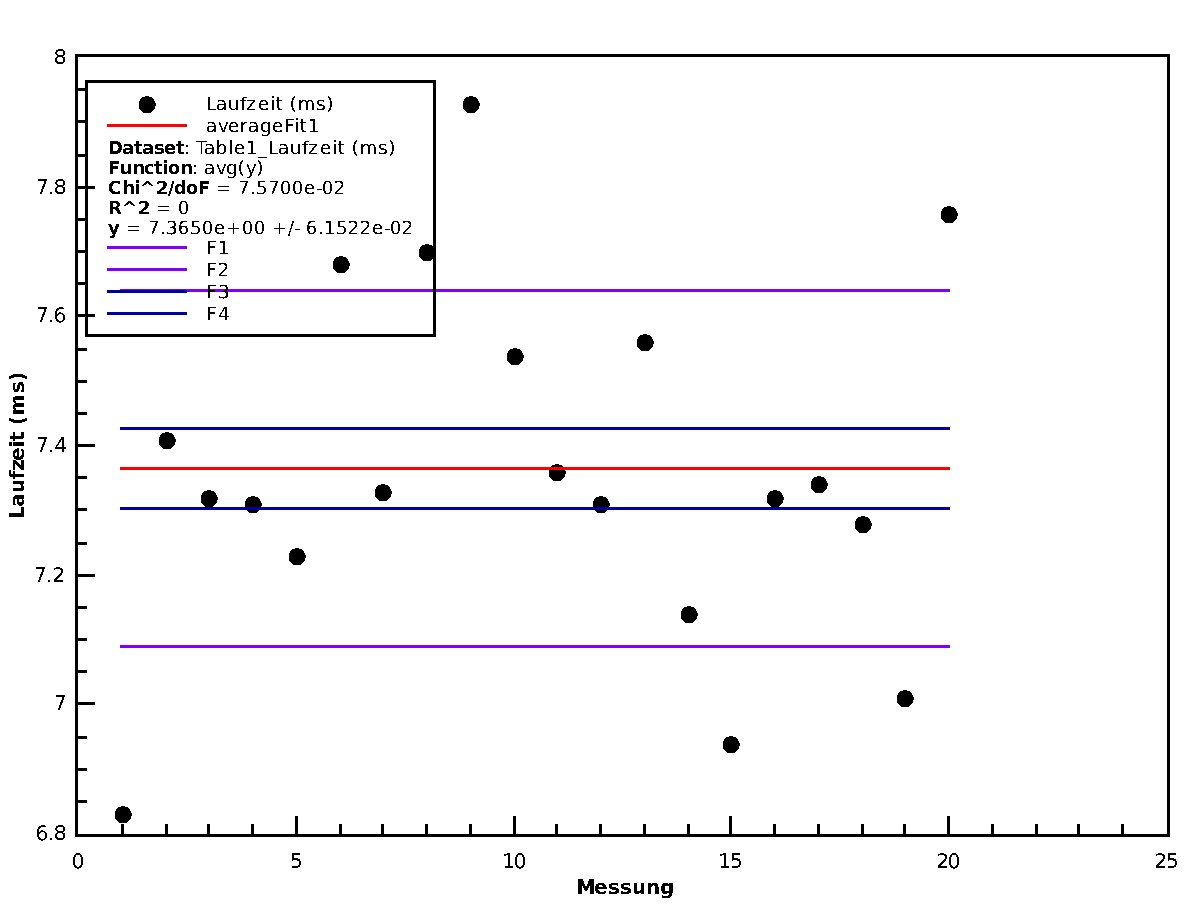
\includegraphics[width=.85\textwidth]{qtiplot/schallgeschwindigkeit}
    \label{fig:schallgeschwindigkeit}
\end{figure}

\subsection{Resultate und Diskussion}

Das Endresultat von $(347.7\pm2.9)\frac{\textrm{m}}{\textrm{s}}$ ist ein wenig h\"oher als der
Literaturwert von $340.29 \frac{\textrm{m}}{\textrm{s}}$. Warscheinlich liegt diese Abweichung
daran, dass der Literaturwert bei $\vartheta=20\degree C$ auf Meeresh\"ohe gemessen wurde
anstatt bei $\vartheta=23\degree C$ (und h\"ochstwarscheinlich auch auf einer anderen H\"ohe). Die
Schallgeschwindigkeit nimmt ab be h\"oherem Druck und tieferer Temperatur ab.

In der Figur \ref{fig:schallgeschwindigkeit} sind die Einzelnen messwerte in einer XY-Scatter-Plot
dargestellt. Die Standardabweichung (Violett) sollte die Stelle markieren, wo statistisch 67\%
aller Messwerte fallen werden. Wenn man nachz\"ahlt, wie viele Punkte innerhalb und ausserhalb des
Bandes liegen -- 13 innerhalb und 8 ausserhalb -- so kommt man grob auf $\frac{8}{13}=\simeq67\textrm{\%}$.

